\section{eo\-Plus\-Replacement$<$ EOT $>$ Class Template Reference}
\label{classeo_plus_replacement}\index{eoPlusReplacement@{eoPlusReplacement}}
ES type of replacement strategy: first add parents to population, then truncate.  


{\tt \#include $<$eo\-Merge\-Reduce.h$>$}

Inheritance diagram for eo\-Plus\-Replacement$<$ EOT $>$::\begin{figure}[H]
\begin{center}
\leavevmode
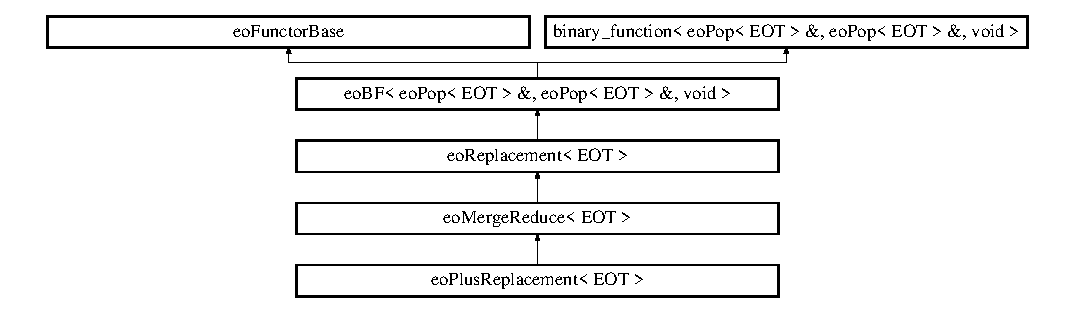
\includegraphics[height=3.76344cm]{classeo_plus_replacement}
\end{center}
\end{figure}
\subsection*{Private Attributes}
\begin{CompactItemize}
\item 
{\bf eo\-Plus}$<$ {\bf EOT} $>$ {\bf plus}\label{classeo_plus_replacement_r0}

\item 
{\bf eo\-Truncate}$<$ {\bf EOT} $>$ {\bf truncate}\label{classeo_plus_replacement_r1}

\end{CompactItemize}


\subsection{Detailed Description}
\subsubsection*{template$<$class EOT$>$ class eo\-Plus\-Replacement$<$ EOT $>$}

ES type of replacement strategy: first add parents to population, then truncate. 



Definition at line 73 of file eo\-Merge\-Reduce.h.

The documentation for this class was generated from the following file:\begin{CompactItemize}
\item 
eo\-Merge\-Reduce.h\end{CompactItemize}
